\documentclass[10pt]{exam}
\usepackage[phy]{template-for-exam}
\usepackage{tikz}
\usetikzlibrary{shadings,decorations.pathmorphing,arrows.meta}

\title{Post-Break Projectile Review}
\author{Rohrbach}
\date{\today}

\begin{document}
\maketitle

\begin{questions}
  
  \question 
    What two things must a \emph{vector} have?
    \vs
  
  \question
    What are the most basic one-dimensional, two-dimensional, and three-dimensional shapes?
    \vs

  \question 
    In the following diagram, label the \emph{resultant} and the \emph{$x$-component}, and the \emph{$y$-component}.

    \vspace{2em}
    \begin{center}
      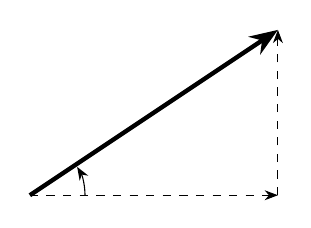
\begin{tikzpicture}[
          every node/.append style={font=\large},
          component/.append style={
            dashed,
            -{Stealth}
          },
          resultant/.append style={
            ultra thick,
            -{Stealth}
          },
          scale=0.7
      ]
        \draw[resultant] 
                  (0,0) -- (4.5,3);
        \draw[component] 
                  (0,0) -- (4.5,0);
        \draw[component] 
                  (4.5,0) -- (4.5,3);
        \draw[-Stealth] (1,0) 
                  arc[
                    start angle = 0,
                    end angle = 31, 
                    radius = 1
                  ];
      \end{tikzpicture}
    \end{center}
    \vspace{2em}

  \question 
    What happens to the $x$-component and $y$-component of a projectile's velocity over time?  
    \vs
    
    
  \question
    Why does this cause the curved shape of the projectile?
    \vs

  \question
    For a given initial projectile speed, which angle gives the furthest range?  Why is that?
    \vs

  \pagebreak

  \question
    \def\velx{16.1}
    \def\vely{42.4}
    Given a projectile with an initial $x$-velocity of \velx~m/s and an intial $y$-velocity of \vely~m/s, fill in the missing velocity measurements on the diagram below

    \vspace{1em}

  \begin{tikzpicture}[
    every node/.append style={font=\footnotesize}
  ]

    \def\apexx{4.5}
    \def\apexy{5}
    \def\vx{\velx/10}
    \def\vy{\vely/10}
    \def\bnk{\fillin[][5em]}

    \draw (-1,-0.7) 
      -- ++(1,0) 
      -- ++(2*\apexx,0) 
      -- ++(1,0);

    \draw[dashed,red] (\apexx,\apexy) 
      coordinate (apex) parabola (0,0);
    \draw[dashed,red] (apex) parabola 
      (2*\apexx,0) coordinate (end);
  
    \draw[ball color=purple] (0,0) circle (0.2);
    \draw[ball color=purple] (apex) circle (0.2);
    \draw[ball color=purple] (end) circle (0.2);


    \draw[dashed, blue] (0,0) -- (\vx, 0)
      node[midway,below=4] {$v_x=\velx$~m/s}
      -- (\vx, \vy)
      node[midway,rotate=90,below=4] {$v_y=\vely$~m/s};
    \draw[ultra thick, blue, ->] (0,0) -- (\vx, \vy)
      node[midway,sloped,above=4] {$v_R=\bnk$};


    \draw[dashed, blue] (end) -- +(\vx, 0)
      node[midway,above=4] {\hspace{2em}$v_x=\bnk$}
      -- +(\vx, -\vy)
      node[midway,rotate=90,below=4] {$v_y=\bnk$};
    \draw[ultra thick, blue, ->] (end) -- +(\vx, -\vy)
      node[midway,sloped,below=4] {$v_R=\bnk$};
  
  
    \draw[ultra thick, blue, ->] (apex) -- ++(\vx,0)
      node[midway,above=5] (lab) {$v_R=\bnk$};
    \node[above of=lab,below=5,blue] (lab2) {$v_y=\bnk$};
    \node[above of=lab2,below=5,blue] (lab2)
      {$v_x=\bnk$};

  \end{tikzpicture}


  \question
    See if you can use kinematic equations to determine the following:

    \begin{tabular}{*{3}{p{10em}}c}
      \\
      \centering $v_f=v_i+at$ &
      \centering $d=v_i t + \tfrac{1}{2} at^2$ &
      \centering $v_f^2 = v_i^2 + 2ad$ & \\
      \centering \it\small ``Old Faithful'' &
      \centering \it\small ``The Big Chalupa'' &
      \centering \it\small ``Ain't Got no Time'' & \\
      \\
    \end{tabular}

    \begin{parts}
      \part Time that the projectile was in the air. \vs
      \part Range ($x$-displacement) of the projectile. \vs
    \end{parts}



 
\end{questions}

\end{document}